% !TeX root = chapter.tex
% Written by Anders Sjoqvist and Ulf Lundstrom, 2009
% The main sources are: tinyKACTL, Beta and Wikipedia

\chapter{Mathematics}

\section{Equations}
\[ax^2+bx+c=0 \Rightarrow x = \frac{-b\pm\sqrt{b^2-4ac}}{2a}\]

The extremum is given by $x = -b/2a$.

\[\begin{aligned}ax+by=e\\cx+dy=f\end{aligned}
\Rightarrow
\begin{aligned}x=\dfrac{ed-bf}{ad-bc}\\y=\dfrac{af-ec}{ad-bc}\end{aligned}\]

In general, given an equation $Ax = b$, the solution to a variable $x_i$ is given by
\[x_i = \frac{\det A_i'}{\det A} \]
where $A_i'$ is $A$ with the $i$'th column replaced by $b$.

\section{Vieta's Formulas}  
For a polynomial of degree \( n \):  
\[
\frac{-b}{a} = \text{sum of roots}, \quad (-1)^n \cdot \frac{k}{a} = \text{product of roots}.
\]  
Here:  
- \( k \) is the coefficient of the constant term,  
- \( a \) is the leading coefficient,  
- \( b \) is the coefficient of the term of degree \( n - 1 \).

\section{Recurrences}
If $a_n = c_1 a_{n-1} + \dots + c_k a_{n-k}$, and $r_1, \dots, r_k$ are distinct roots of $x^k - c_1 x^{k-1} - \dots - c_k$, there are $d_1, \dots, d_k$ s.t.
\[a_n = d_1r_1^n + \dots + d_kr_k^n. \]
Non-distinct roots $r$ become polynomial factors, e.g. $a_n = (d_1n + d_2)r^n$.

\section{Trigonometry}
\begin{align*}
\sin(v+w)&{}=\sin v\cos w+\cos v\sin w\\
\cos(v+w)&{}=\cos v\cos w-\sin v\sin w\\
\tan(v+w)&{}=\dfrac{\tan v+\tan w}{1-\tan v\tan w}\\
\sin v+\sin w&{}=2\sin\dfrac{v+w}{2}\cos\dfrac{v-w}{2}\\
\cos v+\cos w&{}=2\cos\dfrac{v+w}{2}\cos\dfrac{v-w}{2}
\end{align*}
\[ (V+W)\tan(v-w)/2{}=(V-W)\tan(v+w)/2 \]
where $V, W$ are lengths of sides opposite angles $v, w$.
\begin{align*}
	a\cos x+b\sin x&=r\cos(x-\phi)\\
	a\sin x+b\cos x&=r\sin(x+\phi)
\end{align*}
where $r=\sqrt{a^2+b^2}, \phi=\operatorname{atan2}(b,a)$.

\section{Geometry}

\subsection{Triangles}
Side lengths: $a,b,c$\\
Semiperimeter: $p=\dfrac{a+b+c}{2}$\\
Area: $A=\sqrt{p(p-a)(p-b)(p-c)}$\\
Circumradius: $R=\dfrac{abc}{4A}$\\
Inradius: $r=\dfrac{A}{p}$\\
Length of median (divides triangle into two equal-area triangles): $m_a=\tfrac{1}{2}\sqrt{2b^2+2c^2-a^2}$\\
Length of bisector (divides angles in two): $s_a=\sqrt{bc\left[1-\left(\dfrac{a}{b+c}\right)^2\right]}$\\
Law of sines: $\dfrac{\sin\alpha}{a}=\dfrac{\sin\beta}{b}=\dfrac{\sin\gamma}{c}=\dfrac{1}{2R}$\\
Law of cosines: $a^2=b^2+c^2-2bc\cos\alpha$\\
Law of tangents: $\dfrac{a+b}{a-b}=\dfrac{\tan\dfrac{\alpha+\beta}{2}}{\tan\dfrac{\alpha-\beta}{2}}$\\

\subsection{Quadrilaterals}
With side lengths $a,b,c,d$, diagonals $e, f$, diagonals angle $\theta$, area $A$ and
magic flux $F=b^2+d^2-a^2-c^2$:

\[ 4A = 2ef \cdot \sin\theta = F\tan\theta = \sqrt{4e^2f^2-F^2} \]

 For cyclic quadrilaterals the sum of opposite angles is $180^\circ$,
$ef = ac + bd$, and $A = \sqrt{(p-a)(p-b)(p-c)(p-d)}$.

\subsection{Spherical coordinates}
\begin{center}
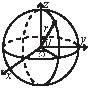
\includegraphics[width=25mm]{content/math/sphericalCoordinates}
\end{center}
\[\begin{array}{cc}
x = r\sin\theta\cos\phi & r = \sqrt{x^2+y^2+z^2}\\
y = r\sin\theta\sin\phi & \theta = \textrm{acos}(z/\sqrt{x^2+y^2+z^2})\\
z = r\cos\theta & \phi = \textrm{atan2}(y,x)
\end{array}\]

\section{Sums}
$c^a + c^{a+1} + \dots + c^{b} = \frac{c^{b+1} - c^a}{c-1}, c \neq 1$
$1 + 2 + 3 + \dots + n = \frac{n(n+1)}{2}$ \\
$1^2 + 2^2 + 3^2 + \dots + n^2 = \frac{n(2n+1)(n+1)}{6}$\\
$1^3 + 2^3 + 3^3 + \dots + n^3 = \frac{n^2(n+1)^2}{4}$ \\
$1^4 + 2^4 + 3^4 + \dots + n^4 = \frac{n(n+1)(2n+1)(3n^2 + 3n - 1)}{30}$ \\

\section{Additional Concepts}

\subsection{Divisors and Sum of Divisors}
    \textbf{Number of Divisors:}  
    If \( N = a^p \times b^q \times \dots \times c^r \), the total number of divisors is:  
    \[
    (p+1) \times (q+1) \times \dots \times (r+1).
    \]  
    \textbf{Sum of Divisors:}  
    For \( N = a^p \times b^q \times \dots \times c^r \), the sum of divisors is:  
    \[
    \text{SumDiv}(N) = \frac{a^{p+1} - 1}{a-1} \cdot \frac{b^{q+1} - 1}{b-1} \cdots \frac{c^{r+1} - 1}{c-1}.
    \]  

\subsection{Sum of an Infinite Geometric Series}  
    The sum of an infinite geometric series of the form:  
    \[
    1 + r + r^2 + r^3 + \ldots = \frac{1}{1 - r}, \quad \text{for } |r| < 1.
    \]

\subsection{Sum of First \( n \) Terms of an AP}
    The sum of the first \( n \) terms (\( S_n \)) is:  
    $S_n = \frac{n}{2} \cdot (2a + (n - 1)d)$

    Alternatively, if the last term (\( l \)) is known:  
    $S_n = \frac{n}{2} \cdot (a + l)$
    Here:  
    - \( S_n \) = sum of the first \( n \) terms,  
    - \( a \) = first term,  
    - \( d \) = common difference,  
    - \( n \) = number of terms,  
    - \( l \) = last term.


\section{Combinatorics}

    \subsubsection{Combinations}  
    
    Without Repetition: $C_{n}^{k}$
    With Repetition: $K_{n}^{k} = \frac{(n + k - 1)!}{k! \cdot (n - 1)!}$
    
    \subsubsection{Arrangements}  
    
    Without Repetition: $A_n^k = \frac{n!}{(n - k)!}$
    With Repetition: $n^k$
    
    \subsubsection{Distributing Identical Objects into Boxes}  
    
    With empty boxes allowed: $C_{n+k-1}^k$
    With no empty box: $C_{n-1}^{k-1}$

    \subsection{Coefficients binomiaux}
    \[
    \binom{n}{k} =
    \begin{cases}
    1 & \text{si } k = 0 \text{ ou } k = n, \\
    \binom{n-1}{k-1} + \binom{n-1}{k} & \text{si } 1 \leq k \leq n-1.
    \end{cases}
    \]
    Somme sur $n$: $\sum_{n = p}^q \binom n k = \binom{q + 1}{k + 1} - \binom{p}{k + 1}$ \newline
    
    \subsection{Principe d'inclusion-exclusion}
    $ | \bigcup_{i \in I} A_i| = \sum_{\substack{J \subset I \\ J \neq \emptyset}} (-1)^{|J| - 1} |\bigcap_{j \in J} A_j| $

\section{Probability theory}
Let $X$ be a discrete random variable with probability $p_X(x)$ of assuming the value $x$. It will then have an expected value (mean) $\mu=\mathbb{E}(X)=\sum_xxp_X(x)$ and variance $\sigma^2=V(X)=\mathbb{E}(X^2)-(\mathbb{E}(X))^2=\sum_x(x-\mathbb{E}(X))^2p_X(x)$ where $\sigma$ is the standard deviation. If $X$ is instead continuous it will have a probability density function $f_X(x)$ and the sums above will instead be integrals with $p_X(x)$ replaced by $f_X(x)$.

Expectation is linear:
Expectation is linear: $\mathbb{E}(aX+bY) = a\mathbb{E}(X)+b\mathbb{E}(Y)$ \\
For independent $X$ and $Y$, $V(aX+bY) = a^2V(X)+b^2V(Y)$

\subsection{Discrete distributions}

\subsubsection{Binomial distribution}
The number of successes in $n$ independent yes/no experiments, each which yields success with probability $p$ is $\textrm{Bin}(n,p),\,n=1,2,\dots,\, 0\leq p\leq1$.
\[p(k)=\binom{n}{k}p^k(1-p)^{n-k}\]
\[\mu = np,\,\sigma^2=np(1-p)\]
$\textrm{Bin}(n,p)$ is approximately $\textrm{Po}(np)$ for small $p$.

\subsubsection{First success distribution}
The number of trials needed to get the first success in independent yes/no experiments, each which yields success with probability $p$ is $\textrm{Fs}(p),\,0\leq p\leq1$.
\[p(k)=p(1-p)^{k-1},\,k=1,2,\dots\]
\[\mu = \frac1p,\,\sigma^2=\frac{1-p}{p^2}\]

\subsection{Continuous distributions}

\subsubsection{Uniform distribution}
If the probability density function is constant between $a$ and $b$ and 0 elsewhere it is $\textrm{U}(a,b),\,a<b$.
\[f(x) = \left\{
\begin{array}{cl}
\frac{1}{b-a} & a<x<b\\
0 & \textrm{otherwise}
\end{array}\right.\]
\[\mu=\frac{a+b}{2},\,\sigma^2=\frac{(b-a)^2}{12}\]
